% fig7-container.tex — Figure 7: Container view (DEV-GOV-03)
%
% What runs, what it keeps on disk, and what is outside the process. The split
% that matters operationally is the top row: MCP servers, hooks and plugins are
% separate processes, so a permission Sego holds is not a permission they hold.
%
% Layout notes: three even columns with wide gaps. An earlier version used 4.8cm
% spacing for boxes that render about 4.8cm wide, which put every box on top of
% its neighbour, and routed the external arrows from inner nodes so that they
% crossed the whole figure. Arrows now meet the process boundary instead.
\documentclass[tikz,border=10pt]{standalone}
\usetikzlibrary{arrows.meta,positioning,fit,backgrounds,calc}

\begin{document}
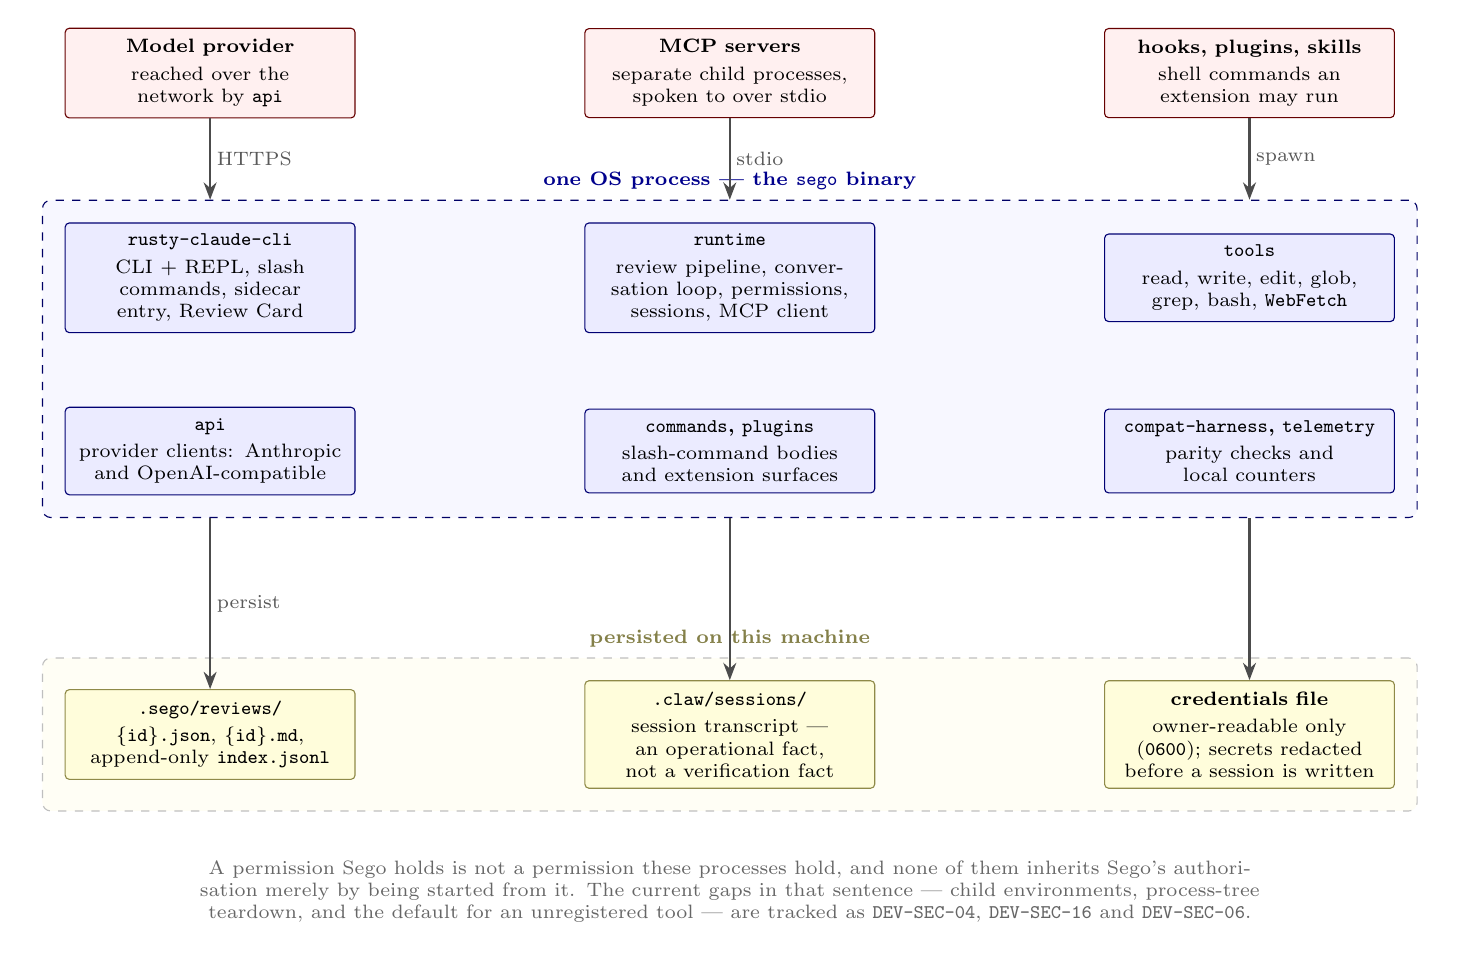
\begin{tikzpicture}[
  x=1cm, y=1cm,
  font=\small,
  crate/.style={draw, rounded corners=1.5pt, fill=blue!8, draw=blue!45!black,
                font=\scriptsize, align=center, inner sep=4pt, text width=34mm},
  store/.style={draw, rounded corners=1.5pt, fill=yellow!14, draw=yellow!50!black,
                font=\scriptsize, align=center, inner sep=4pt, text width=34mm},
  ext/.style={draw, rounded corners=1.5pt, fill=red!6, draw=red!40!black,
              font=\scriptsize, align=center, inner sep=4pt, text width=34mm},
  arr/.style={-{Stealth[length=2.2mm]}, thick, draw=black!70},
  lab/.style={font=\scriptsize, text=black!65, inner sep=2pt, fill=white},
  grp/.style={draw=black!25, dashed, rounded corners=3pt, inner sep=8pt},
  zone/.style={draw=blue!40!black, dashed, rounded corners=3pt, inner sep=8pt}
]

% ---------------- outside the process ----------------
\node[ext] (prov) at (-6.6, 6.0)
  {\textbf{Model provider}\\[2pt] reached over the network by \texttt{api}};
\node[ext] (mcp) at (0, 6.0)
  {\textbf{MCP servers}\\[2pt] separate child processes, spoken to over stdio};
\node[ext] (hook) at (6.6, 6.0)
  {\textbf{hooks, plugins, skills}\\[2pt] shell commands an extension may run};

% ---------------- the process ----------------
\node[crate] (cli) at (-6.6, 3.4)
  {\textbf{\texttt{rusty-claude-cli}}\\[2pt] CLI + REPL, slash commands, sidecar entry, Review Card};
\node[crate] (rt) at (0, 3.4)
  {\textbf{\texttt{runtime}}\\[2pt] review pipeline, conversation loop, permissions, sessions, MCP client};
\node[crate] (tools) at (6.6, 3.4)
  {\textbf{\texttt{tools}}\\[2pt] read, write, edit, glob, grep, bash, \texttt{WebFetch}};
\node[crate] (api) at (-6.6, 1.2)
  {\textbf{\texttt{api}}\\[2pt] provider clients: Anthropic and OpenAI-compatible};
\node[crate] (cmd) at (0, 1.2)
  {\textbf{\texttt{commands}, \texttt{plugins}}\\[2pt] slash-command bodies and extension surfaces};
\node[crate] (harness) at (6.6, 1.2)
  {\textbf{\texttt{compat-harness}, \texttt{telemetry}}\\[2pt] parity checks and local counters};

\begin{scope}[on background layer]
  \node[zone, fill=blue!3,
        label={[font=\scriptsize\bfseries, text=blue!55!black]above:one OS process --- the \texttt{sego} binary}]
    (proc) [fit=(cli)(rt)(tools)(api)(cmd)(harness)] {};
\end{scope}

% ---------------- persisted ----------------
\node[store] (reviews) at (-6.6, -2.4)
  {\textbf{\texttt{.sego/reviews/}}\\[2pt] \texttt{\{id\}.json}, \texttt{\{id\}.md}, append-only \texttt{index.jsonl}};
\node[store] (sessions) at (0, -2.4)
  {\textbf{\texttt{.claw/sessions/}}\\[2pt] session transcript --- an operational fact, not a verification fact};
\node[store] (creds) at (6.6, -2.4)
  {\textbf{credentials file}\\[2pt] owner-readable only (\texttt{0600}); secrets redacted before a session is written};

\begin{scope}[on background layer]
  \node[grp, fill=yellow!4,
        label={[font=\scriptsize\bfseries, text=yellow!45!black]above:persisted on this machine}]
    (disk) [fit=(reviews)(sessions)(creds)] {};
\end{scope}

% ---------------- arrows meet the boundary ----------------
\draw[arr] (prov.south) -- node[lab, right] {HTTPS} (proc.north -| prov);
\draw[arr] (mcp.south) -- node[lab, right] {stdio} (proc.north -| mcp);
\draw[arr] (hook.south) -- node[lab, right] {spawn} (proc.north -| hook);
\draw[arr] (proc.south -| reviews) -- node[lab, right] {persist} (reviews.north);
\draw[arr] (proc.south -| sessions) -- (sessions.north);
\draw[arr] (proc.south -| creds) -- (creds.north);

\node[font=\scriptsize, text=black!60, text width=176mm, align=center] at (0, -4.4)
  {A permission Sego holds is not a permission these processes hold, and none of them inherits Sego's authorisation merely by
   being started from it. The current gaps in that sentence --- child environments, process-tree teardown, and the default for
   an unregistered tool --- are tracked as \texttt{DEV-SEC-04}, \texttt{DEV-SEC-16} and \texttt{DEV-SEC-06}.};

\end{tikzpicture}
\end{document}
